\documentclass[tikz,border=12pt]{standalone}
\usepackage{amsmath}
\usepackage{tikz}
\usetikzlibrary{3d,shapes.geometric,arrows.meta,calc}

\begin{document}
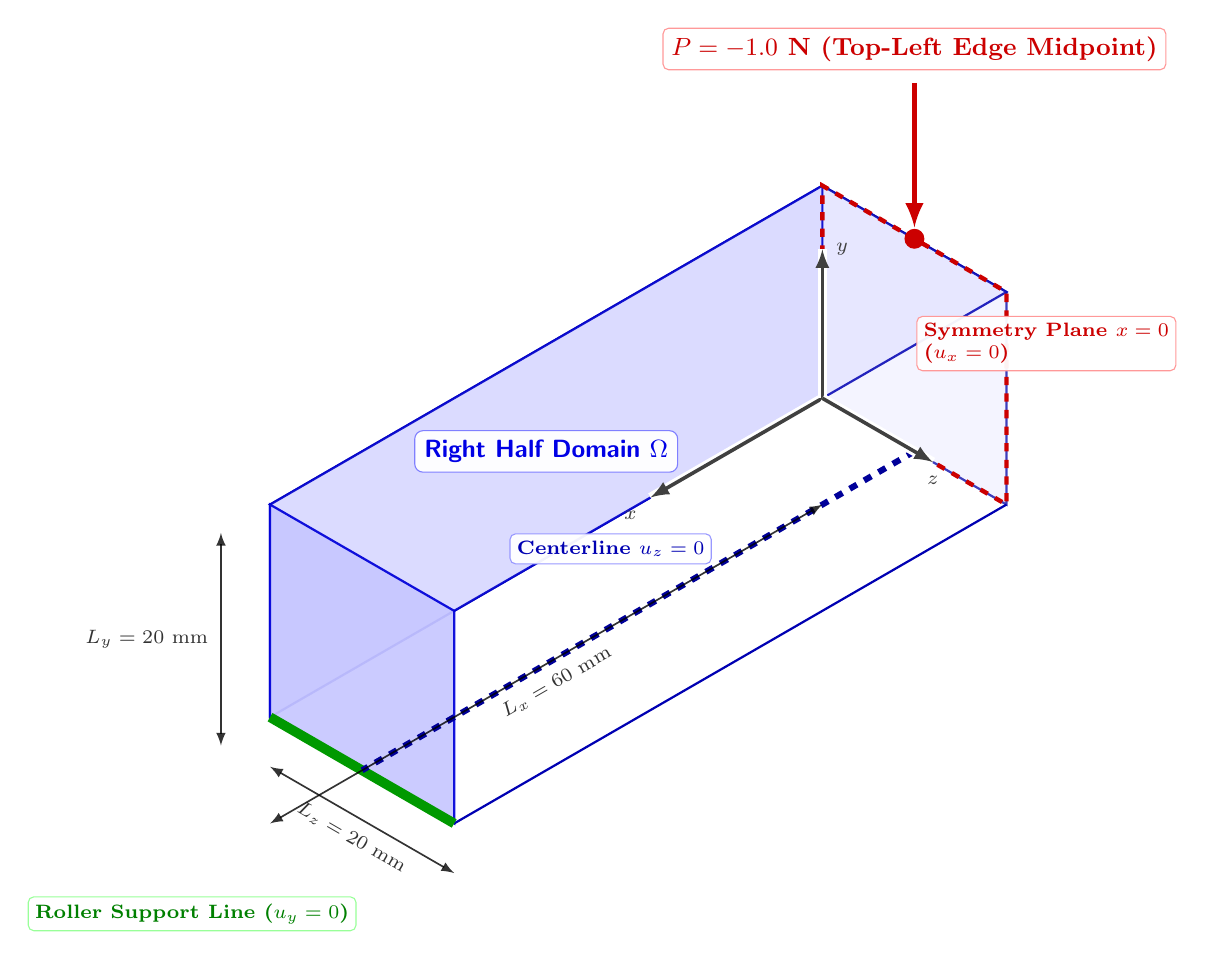
\begin{tikzpicture}[x={(-0.866cm,-0.5cm)}, y={(0.866cm,-0.5cm)}, z={(0cm,1cm)}, scale=1.8, >=latex]
  % ============================================================
  % 坐标映射 (与 HalfMBBBeamRight3d 代码坐标系精确一致):
  %   TikZ x = 代码 x = 长度 Lx = 60 mm (右半域)
  %   TikZ y = 代码 z = 宽度 Lz = 20 mm (屏幕右下方向)
  %   TikZ z = 代码 y = 高度 Ly = 20 mm (屏幕竖直方向)
  % 版式沿用 mbb_3d_full_beam.tex, 只把左端面换成对称面。
  % ============================================================
  \def\Lx{4.5}
  \def\Ly{1.5}   % 宽度 (代码 z)
  \def\Lz{1.5}   % 高度 (代码 y)

  % 1. Draw 3D Box Faces (Back-to-Front ordering)

  % 左端面 = 对称面 (代码 x=0)
  \draw[thick, fill=blue!6, draw=blue!65!black, opacity=0.75]
    (0,0,0) -- (0,\Ly,0) -- (0,\Ly,\Lz) -- (0,0,\Lz) -- cycle;

  % 顶面 (代码 y=L_y, TikZ z=\Lz)
  \draw[thick, fill=blue!10, draw=blue!70!black, opacity=0.85]
    (0,0,\Lz) -- (\Lx,0,\Lz) -- (\Lx,\Ly,\Lz) -- (0,\Ly,\Lz) -- cycle;

  % 前面 (代码 z=0, TikZ y=0)
  \draw[thick, fill=blue!15, draw=blue!80!black, opacity=0.9]
    (0,0,0) -- (\Lx,0,0) -- (\Lx,0,\Lz) -- (0,0,\Lz) -- cycle;

  % 右端面 (代码 x=L_x, TikZ x=\Lx)
  \draw[thick, fill=blue!22, draw=blue!85!black, opacity=0.92]
    (\Lx,0,0) -- (\Lx,\Ly,0) -- (\Lx,\Ly,\Lz) -- (\Lx,0,\Lz) -- cycle;

  % 底面后缘棱线
  \draw[thick, draw=blue!70!black] (0,\Ly,0) -- (\Lx,\Ly,0);

  % 2. Domain Label (前面板中心)
  \node[font=\small\bfseries\sffamily, color=blue!90!black,
        fill=white, fill opacity=0.95, text opacity=1.0, inner sep=3.5pt, rounded corners=3pt, draw=blue!50]
        at (\Lx*0.5, 0, \Lz*0.5) {Right Half Domain $\Omega$};

  % 3. 对称面 (代码 x=0 整个左端面): u_x = 0
  \draw[ultra thick, red!80!black, dashed]
    (0,0,0) -- (0,\Ly,0) -- (0,\Ly,\Lz) -- (0,0,\Lz) -- cycle;
  \node[above right=4pt, red!80!black, font=\scriptsize\bfseries, align=left,
        fill=white, fill opacity=0.95, text opacity=1.0, inner sep=2.5pt, rounded corners=2pt, draw=red!40]
        at (0, \Ly*0.45, \Lz*0.30) {Symmetry Plane $x=0$\\($u_x = 0$)};

  % 4. 滚轴支座线 (代码: u_y = 0 于 x=Lx, y=0, 沿 z 宽度)
  \draw[line width=3.5pt, green!60!black] (\Lx,0,0) -- (\Lx,\Ly,0);
  \node[below left=2pt, green!50!black, font=\scriptsize\bfseries, align=center,
        fill=white, fill opacity=0.95, text opacity=1.0, inner sep=2.5pt, rounded corners=2pt, draw=green!40]
        at (\Lx, \Ly*0.5, -0.85) {Roller Support Line ($u_y = 0$)};

  % 5. u_z = 0 底面中心线 (代码: y=0, z=Lz/2, 沿 x 长度) —— 消去面外刚体平动
  \draw[line width=2.2pt, blue!60!black, dashed] (0,\Ly*0.5,0) -- (\Lx,\Ly*0.5,0);
  \node[blue!70!black, font=\scriptsize\bfseries, align=center,
        fill=white, fill opacity=0.95, text opacity=1.0, inner sep=2.5pt, rounded corners=2pt, draw=blue!40]
        at (\Lx*0.55, \Ly*0.5, 0.55) {Centerline $u_z = 0$};

  % 6. 集中力 P = -1.0 N 于对称面顶棱中点 (代码: x=0, y=Ly, z=Lz/2)
  \coordinate (TopLeft) at (0, \Ly/2, \Lz);
  \fill[red!80!black] (TopLeft) circle (2.0pt);
  \draw[->, ultra thick, red!80!black, line width=2.0pt]
    (0, \Ly/2, \Lz+1.1) -- (0, \Ly/2, \Lz+0.08);
  \node[above=2pt, red!80!black, font=\small\bfseries,
        fill=white, fill opacity=0.95, text opacity=1.0, inner sep=3pt, rounded corners=2pt, draw=red!40]
        at (0, \Ly/2, \Lz+1.15) {$P = -1.0\text{ N}$ (Top-Left Edge Midpoint)};

  % 7. 坐标轴 (原点: 左前下角)
  \draw[line width=3.4pt, white] (0,0,0) -- (1.4,0,0);
  \draw[->, line width=1.3pt, black!75] (0,0,0) -- (1.4,0,0)
    node[below left=1pt, black!75, font=\scriptsize\bfseries] {$x$};
  \draw[line width=3.4pt, white] (0,0,0) -- (0,0,1.05);
  \draw[->, line width=1.3pt, black!75] (0,0,0) -- (0,0,1.05)
    node[right=1pt, black!75, font=\scriptsize\bfseries] {$y$};
  \draw[line width=3.4pt, white] (0,0,0) -- (0,0.9,0);
  \draw[->, line width=1.3pt, black!75] (0,0,0) -- (0,0.9,0)
    node[below=1pt, black!75, font=\scriptsize\bfseries] {$z$};

  % 8. Dimension Lines (全部布置在实体之外)
  \draw[<->, opacity=0.8, semithick] (0,0,-0.75) -- (\Lx,0,-0.75)
    node[midway, sloped, below=1pt, font=\scriptsize] {$L_x = 60\text{ mm}$};
  \draw[<->, opacity=0.8, semithick] (\Lx+0.4,0,0) -- (\Lx+0.4,0,\Lz)
    node[midway, left=1pt, font=\scriptsize] {$L_y = 20\text{ mm}$};
  \draw[<->, opacity=0.8, semithick] (\Lx,0,-0.35) -- (\Lx,\Ly,-0.35)
    node[midway, sloped, below=1pt, font=\scriptsize] {$L_z = 20\text{ mm}$};
\end{tikzpicture}
\end{document}
